\selectlanguage{portuguese}
\begin{multicols}{2}
  \cappar O meu nome é Sérgio Miguel, nascido em Luanda,
  Angola. Cresci na Cazenga periférica. Pertenço a uma grande família
  que consta de quatro irmãos e duas irmãs. Como para muitas crianças,
  os jogos fizeram sempre parte da vida das crianças do meu bairro.
  Posso recordar o jogo da Buraca, a semalha, da saída de bote e
  muitos outros. Na década de 90, os jogos foram sempre elementos de
  recriação e socialização muito comum nos bairros de Luanda. Aprendi
  a jogar xadrez com 12 anos de idade. Antes de jogar damas com o meu
  irmão gémeo, o xadrez levou à complexidade e à riqueza de ideias de
  que careciam as damas.

 \begin{figurebox}
     \centering
    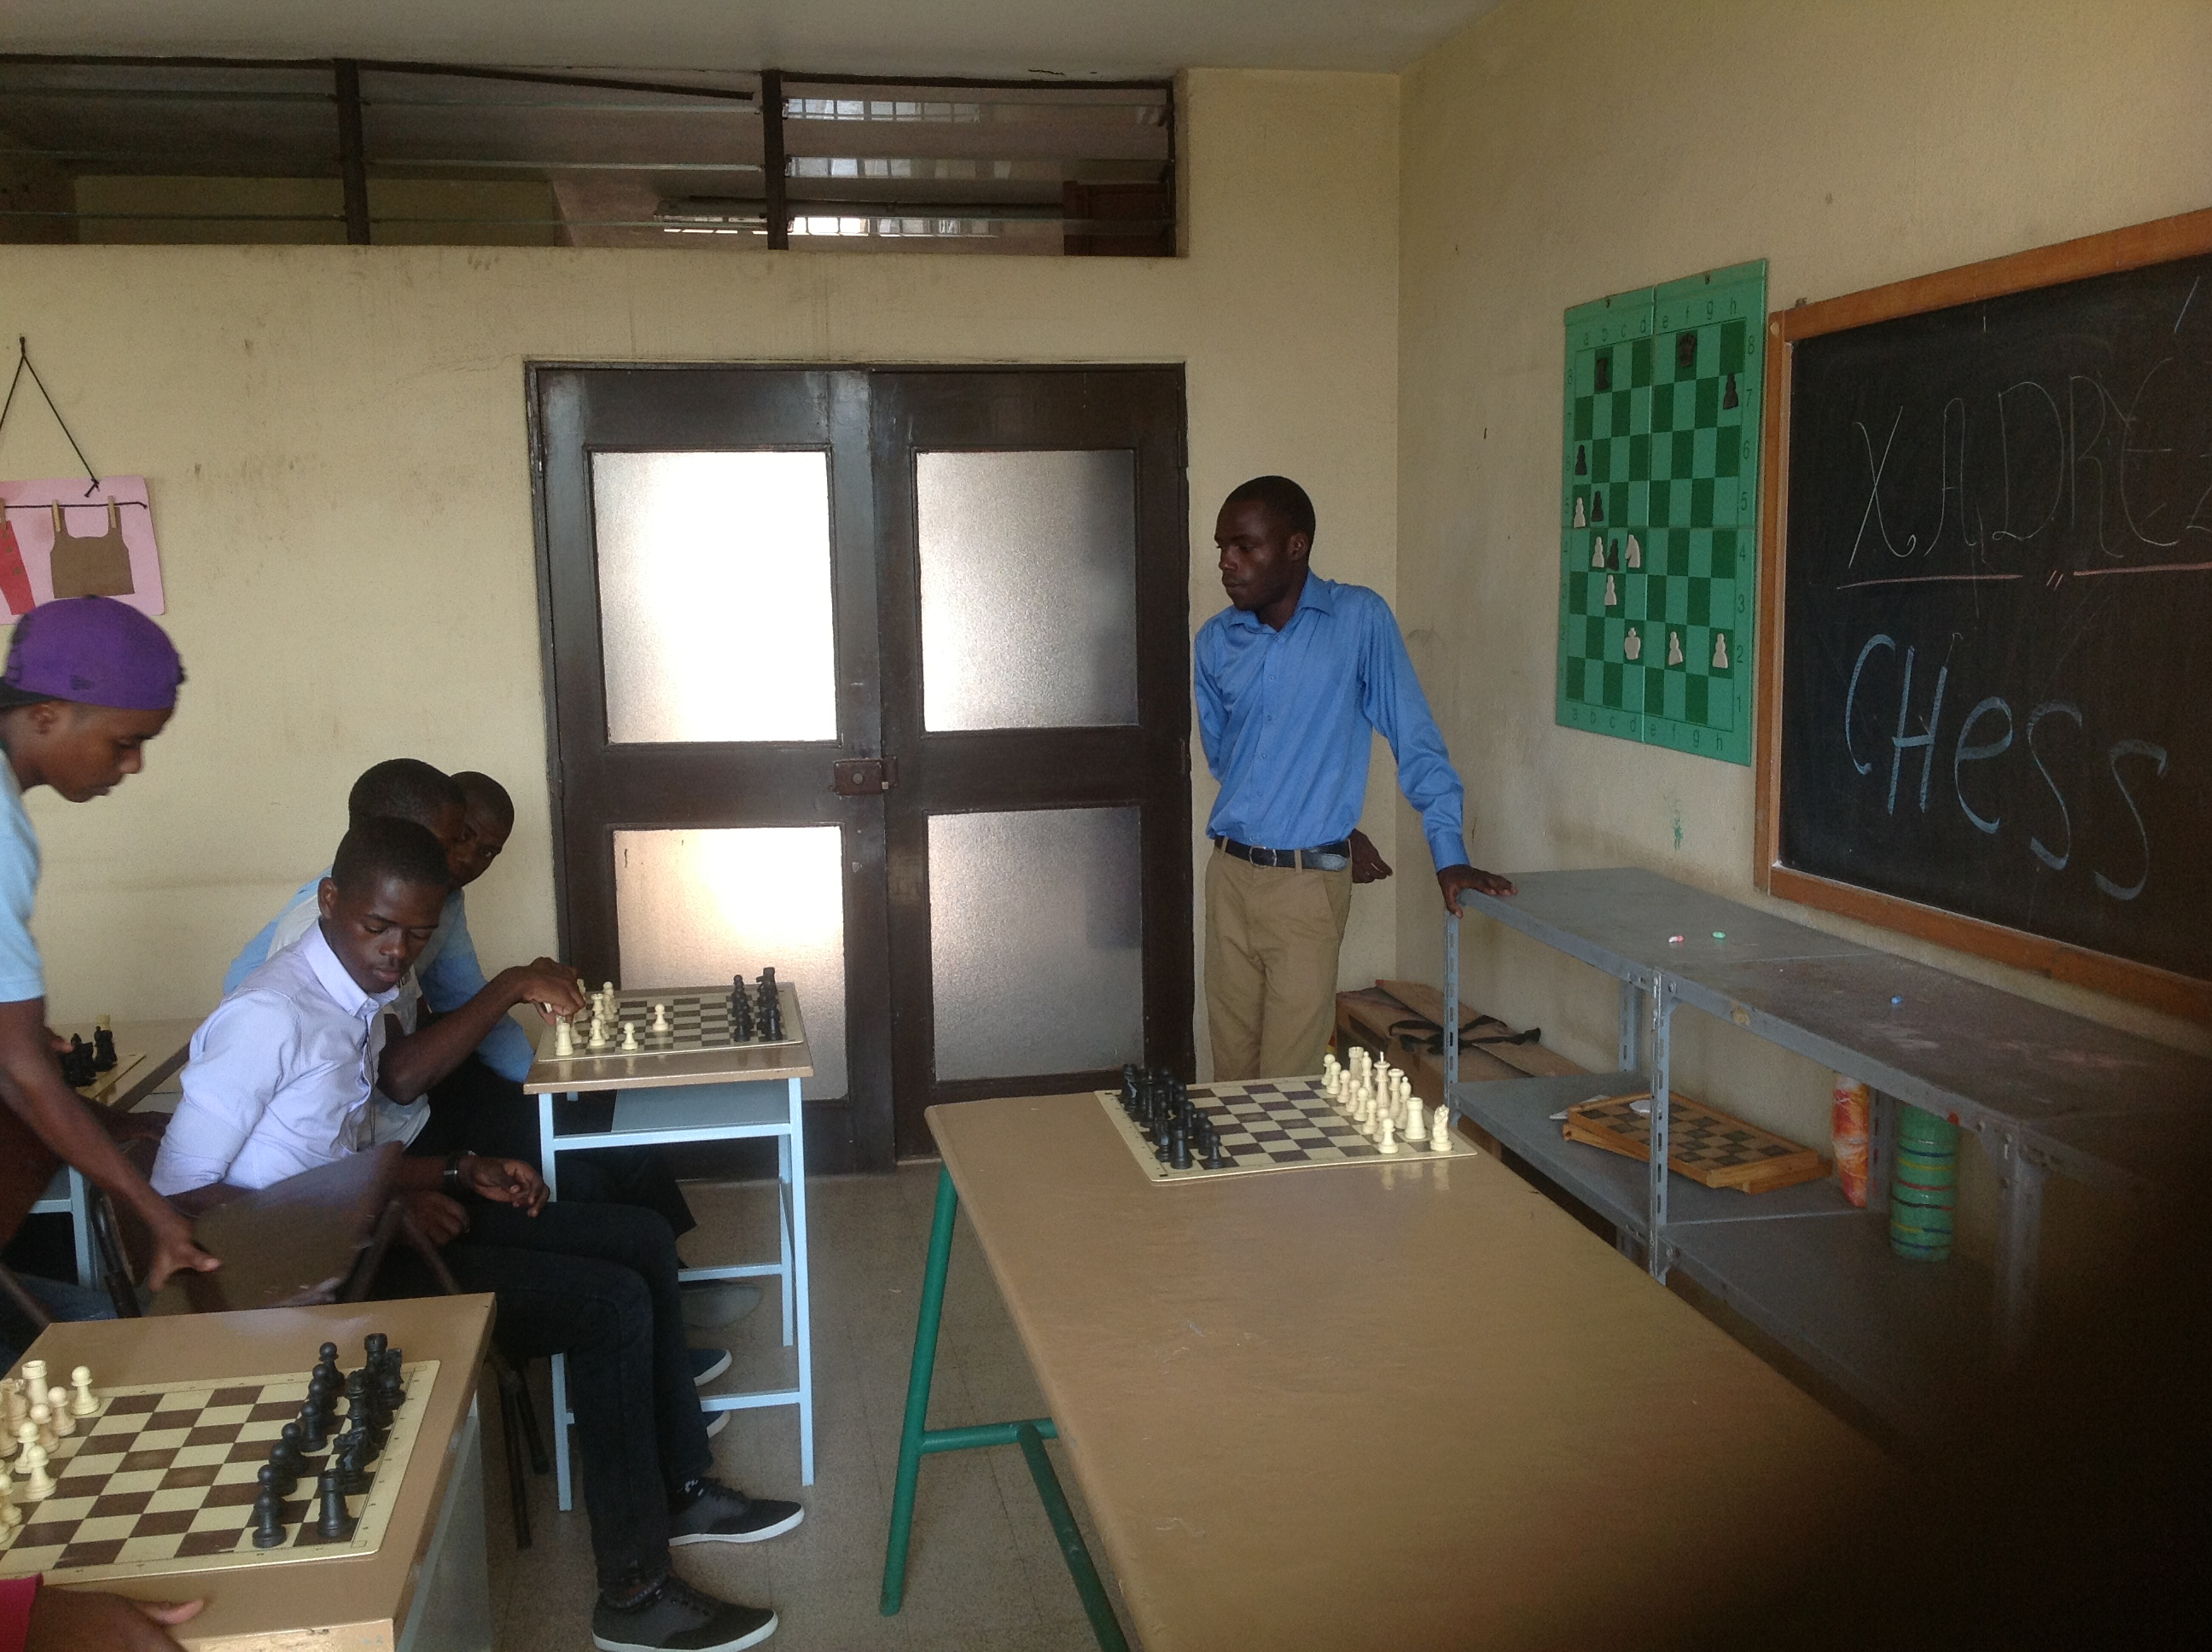
\includegraphics[scale=0.09]{IMG_4774.JPG}\\
    Sérgio Miguel Cabila       
  \end{figurebox}

Com 18 anos de idade visitei a escola de xadrez do meu condado. A minha motivação era
simplesmente saber mais sobre o jogo e fazer amigos. No clube do
caminho Cazenga encontrei os primeiros jogadores realmente
difíceis. Surpreendentemente, depois de vencer no torneio nacional, fui
convocado para representar o clube no campeonato provincial de
xadrez, e desta forma comecei a praticar xadrez profissional.

Fui campeão de xadrez da província de Luanda em 2012 e subcampeão
nacional, no mesmo ano pediram-me para representar a seleção
de Angola nos Jogos Olímpicos, onde obtive o título de CM
(candidato a mestre). Além de viajar pelas diversas províncias de
Angola, tive a oportunidade de conhecer países como Portugal, Tunísia,
Turquia, França e Espanha.
 
 \begin{figurebox}
     \centering
    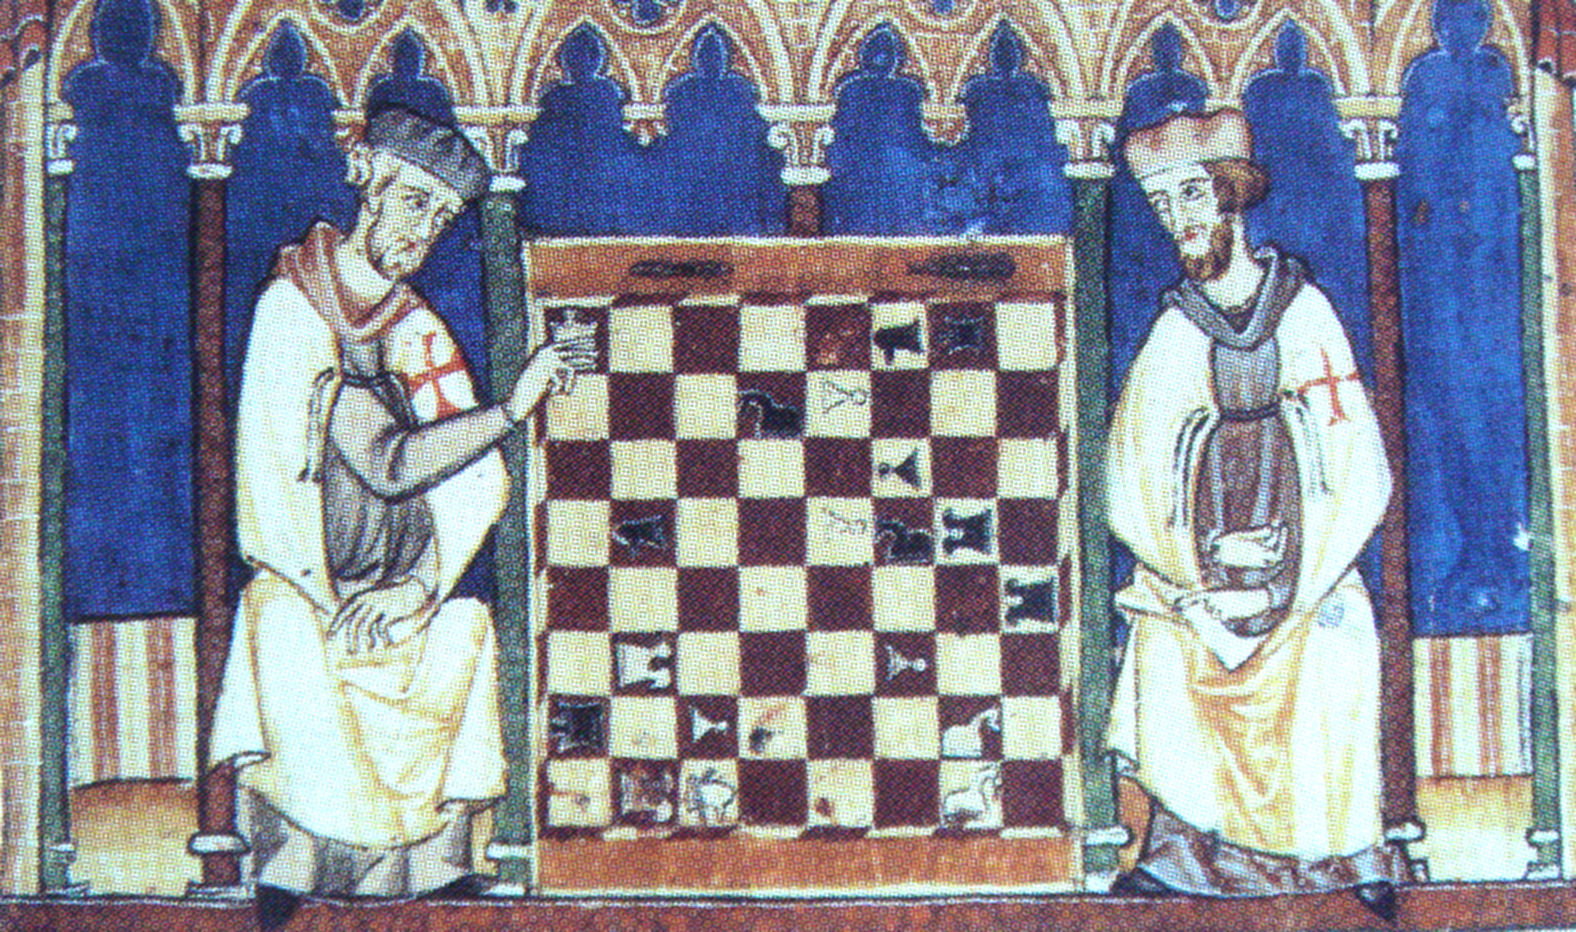
\includegraphics[scale=0.15]{libro.jpg}
     \end{figurebox}


     Sou professor de xadrez e atualmente dou 3 aulas em 2 escolas
     diferentes, a primeira é um turma de adolescentes de 14 a 20 anos
     de idade. Na escola marista em INME o clube de xadrez é uma opção
     dentro deste desporto. Em oito anos ensinaram a cerca de 300
     estudantes. Em LIS (Luanda internacional Scholl) iniciaram uma
     aula de crianças de 1 ano letivo para crianças com 6 a 12 anos de
     idade. Ensinamos em Inglês. E, mais recentemente, trabalhámos o
     projeto Carisma que tem como objetivo fazer uma monitorização de
     múltiplas facetas na vida dos estudantes para envolver aos pais
     interessados em ver os seus filhos com um desenvolvimento
     especial no jogo do xadrez.

     A metodologia utilizada varia de estudante para
     estudante. Utilizamos software para apresentar rapidamente um
     tema particular de combinações particulares, como ver os
     estudantes na prática, porque julgo que o xadrez deve ser um
     elemento de socialização e ligação entre os estudantes. Os
     estudantes mais experientes consolidam os seus conhecimentos à
     medida que ensinam os menos experientes. Também fizemos uma
     análise de partidas, teses, torneios temáticos, etc.

 \begin{figurebox}
     \centering
        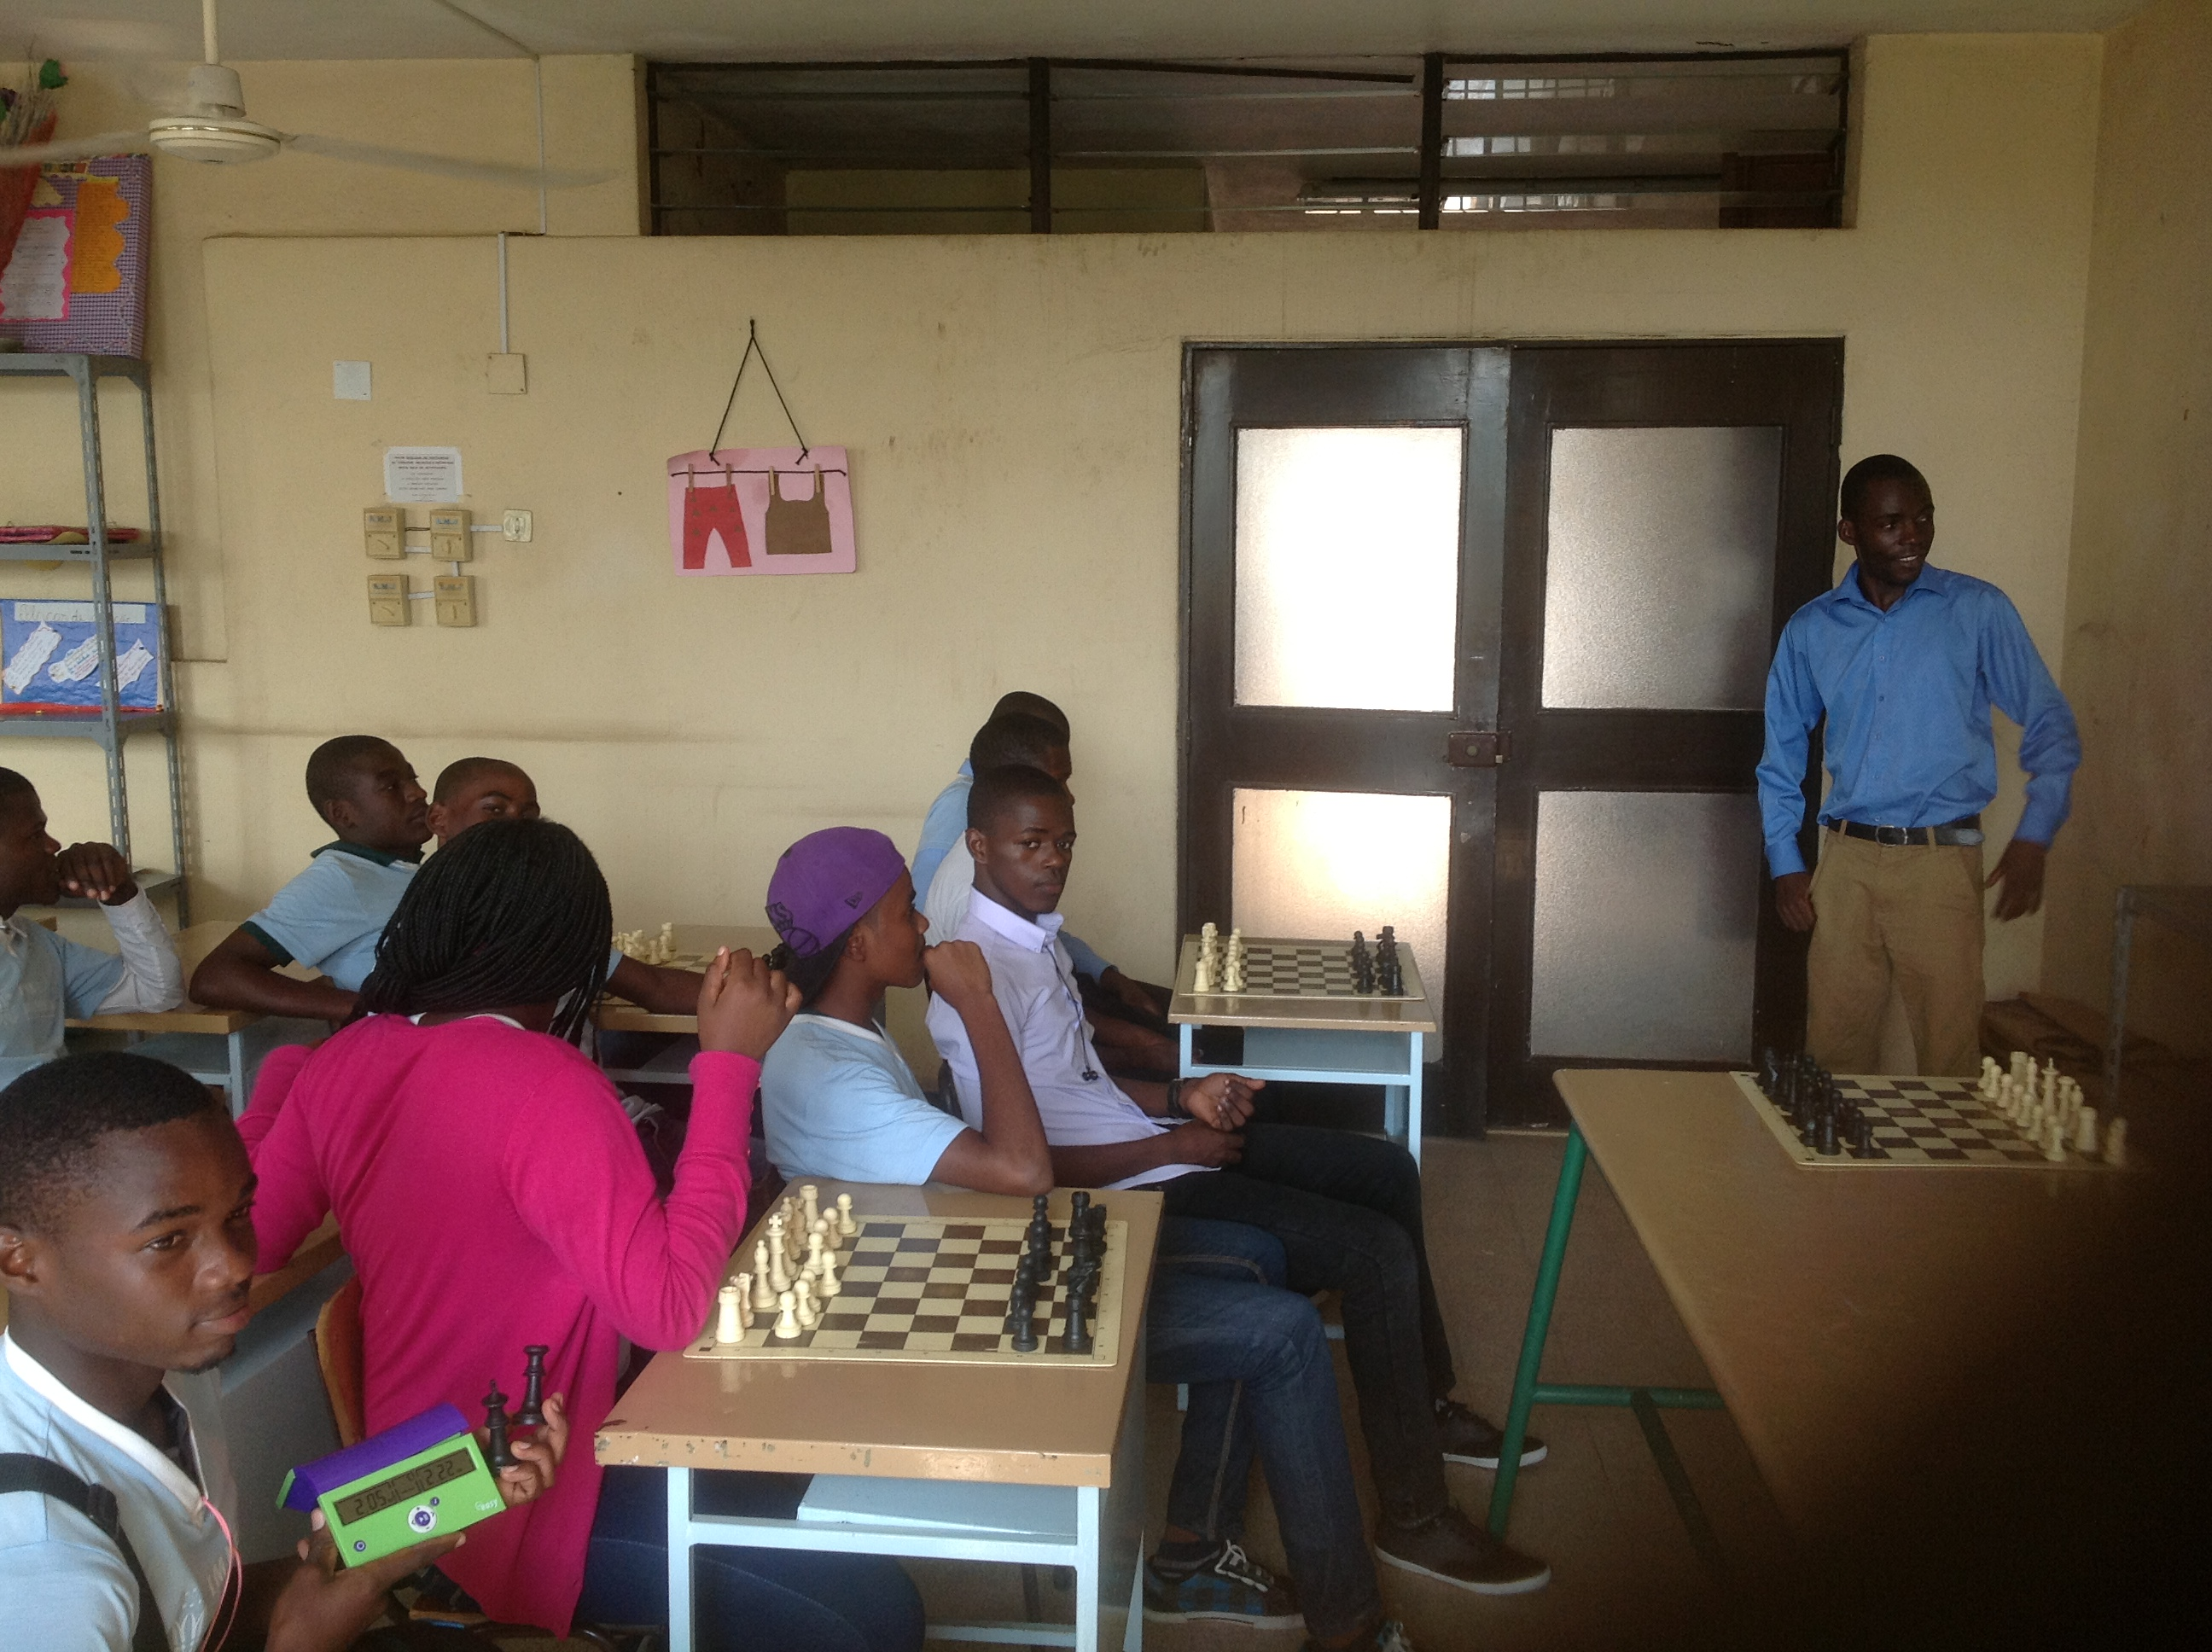
\includegraphics[scale=0.09]{IMG_4775.JPG}
  \end{figurebox}
\vspace{-3cm}


Incentivar os alunos é um desafio constante e está-se constantemente à
procura de soluções face a este problema, em essência, primeiro tenho
o cuidado de lhes dar a conhecer os problemas que encontram no seu
caminho. Sempre que se apercebam do problema, na maioria dos casos
para entender o que se está a passar, o que participam as partes e a
posição que ocupam, é suficiente. Quando faltar alguma coisa depois
dividem o problema pelas partidas mais pequenas, tais como perguntas;
encontrar as peças indefensas? Quantas possibilidades existem de fazer
xeques? Muita ajuda para os meus estudantes. Os temas que estão ao seu
alcance são os que se adaptam à sua aprendizagem para manter a
motivação. A sensação que tenho quando depois de alguns minutos se
pode resolver um problema que parecia insolúvel, é grande satisfação e
motivação, quer do estudante quer do professor.


 \begin{figurebox}
     \centering
       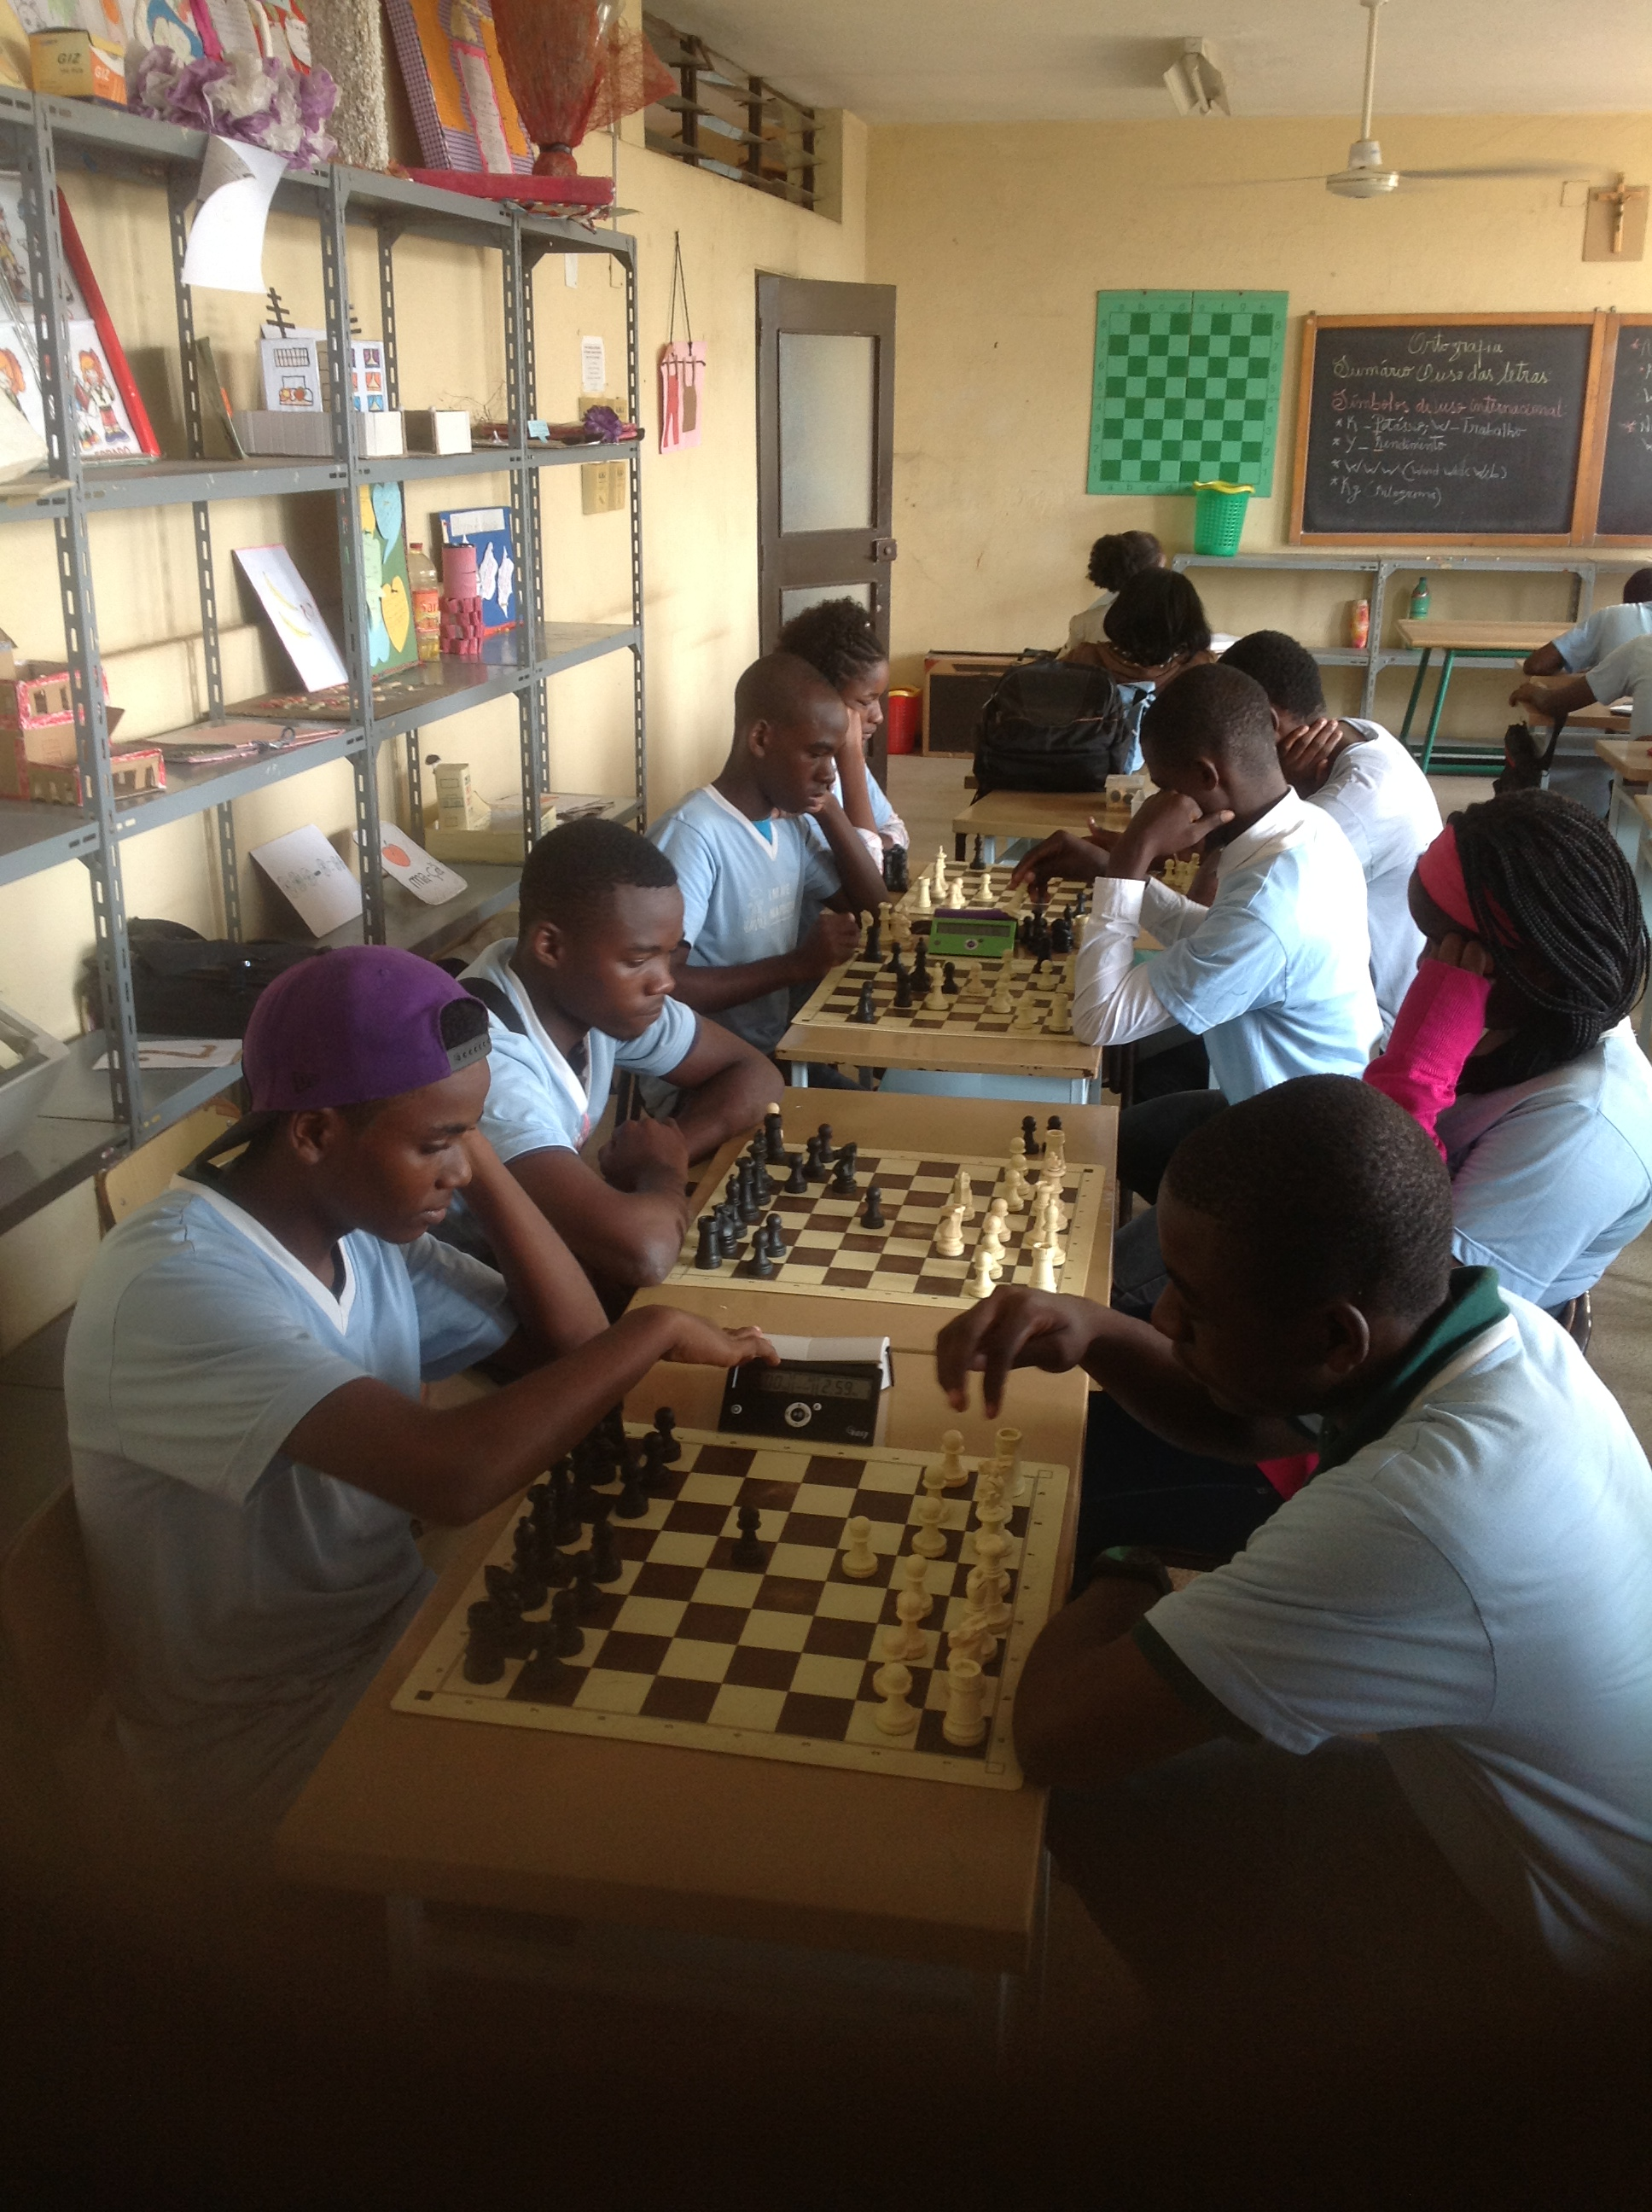
\includegraphics[scale=0.06]{IMG_4768.JPG}
    \end{figurebox}


Gostaria de me despedir com uma mensagem para o povo angolano.
Com a chegada da paz,  Angola tem experimentado um forte
crescimento económico nos últimos anos. A educação é a base de
um verdadeiro desenvolvimento. Vemos como muitas outras escolas são construídas e
reabilitadas. Acredito na educação como uma cultura, como uma fruta
que deve amadurecer. A verdadeira educação em valores do ser humano acima
dos bens materiais, tem como objetivo o desenvolvimento do homem
em todas as dimensões. O homem está acima do dinheiro,
devemos considerar ser mais do que ter. Uma educação transformadora que
responde à formação íntegra do homem na vida social,
recursos humanos, materiais e dimensões espirituais. Que o povo
de Angola aprenda a desfrutar dos bens e da beleza do
país e saibamos que a maior riqueza de uma nação são as pessoas a
aprenderem a viver e deixar que os outros vivam. Desfrutar umas das
outras. E estes valores devem ser defendidos pela Educação. A
integração do desporto escolar e do xadrez em particular contribui
para uma educação moderna, baseada no desenvolvimento íntegro. Desenvolver
nos estudantes a capacidade de pensar, resolver problemas e o
raciocínio em vez de simplesmente receber informação.

\end{multicols}
\newpage
%%% Local Variables: 
%%% mode: latex
%%% TeX-master: "nadaesimposible"
%%% End: 


